\documentclass[12pt,a4paper]{article}
\usepackage[utf8]{inputenc}
\usepackage[T1]{fontenc}
\usepackage[ngerman]{babel}
\usepackage{csquotes}
\usepackage[backend=biber,style=authoryear,maxcitenames=2,maxbibnames=99]{biblatex}
\addbibresource{Organisation.bib} % Bib-Datei nicht vergessen!
\newcommand{\zitat}[1]{\parencite{#1}}
\bibliography{Organisation}
\usepackage{geometry}
\geometry{
	left=30mm,
	right=30mm,
	top=25mm,
	bottom=25mm
}
\usepackage{graphicx}
\usepackage{float}
\usepackage{setspace}
\onehalfspacing
\usepackage{caption}
\usepackage{tocloft}
\usepackage{hyperref}
\hypersetup{colorlinks=true, linkcolor=black, urlcolor=blue, citecolor=black}
\usepackage{acronym}
\usepackage[nottoc]{tocbibind}
\usepackage{etoolbox} % für robusten Befehl
\usepackage{lipsum} % nur für Blindtext, kann entfernt werden
\usepackage{setspace} % für Zeilenabstand
\usepackage{ragged2e} % für \justifying


\newcommand{\absatzZitat}[1]{%
	\begin{quote}
		\fontsize{10pt}{12pt}\selectfont
		\setstretch{1.0}
		\leftskip=1cm
		\rightskip=1cm
		\justifying
		#1
	\end{quote}
}

\begin{document}
	
	%------------------------- Titelseite -------------------------
	\begin{titlepage}
		\centering
		\vfill
		{\Huge \textbf{Deutsche Telekom}}\\[1.5cm]
		\large
		Seminar: Grundlagen der Organisation\\
		Sommersemester 2025\\[2cm]
		
\includegraphics[width=0.4\textwidth]{images/UOL-Logo.png}\\[2cm]
		\normalsize
		\begin{flushleft}
			\textbf{Betreurin:} Prof. Dr. Julia Brennecke\\[0.5cm]
			\textbf{Abgegeben von:}\\
			Mika Scheinig\\
			Elija Wendte\\
			Justus Kressmann\\
			Engin Fidansoy\\
			Manar Krenbeh\\[0.5cm]
			Carl von Ossietzky Universität Oldenburg\\
			Fakultät II – Informatik, Wirtschafts- und Rechtswissenschaften\\
		\end{flushleft}
		\vfill
		\begin{flushright}
			Abgabedatum: 01. Juni 2025
		\end{flushright}
	\end{titlepage}
	
	%------------------------- Eidesstattliche Erklärung -------------------------
	\pagenumbering{Roman}
	
	\section*{\texorpdfstring{Executive Summary}{Executive Summary }}\label{executive-summary}
	
	In diesem Bericht wird die Aufbau- und Ablauforganisation der Deutschen
	Telekom AG untersucht, die mit rund 200.000 Mitarbeitenden in mehr als
	50 Ländern zu den größten Telekommunikationsanbietern weltweit gehört.
	Der Konzern organisiert sich im Wesentlichen divisional, wobei
	Matrixelemente in Bereichen wie IT, Personal und Strategie hinzukommen.
	Diese hybride Struktur soll Spezialisierung, Kund:innennähe und
	Flexibilität ermöglichen. Allerdings ergeben sich dabei auch
	Schwierigkeiten bei Koordination, Abstimmung und der Bestimmung
	eindeutiger Zuständigkeiten. Die Analyse legt offen, dass interne
	Abläufe teils als schwerfällig wahrgenommen werden.
	Entscheidungsprozesse nehmen viel Zeit in Anspruch, interdisziplinäre
	Kooperation funktioniert nicht optimal, und Silo-Denken erschwert eine
	übergreifende Sichtweise. Agile Arbeitsformen lassen sich unter diesen
	Bedingungen schwer integrieren. Bestehende Initiativen wie digitale
	Lernplattformen, neue Führungsmodelle und bereichsübergreifende Projekte
	sind wichtige Schritte, reichen jedoch nicht aus, um strukturelle
	Schwächen zu beheben.
	
	\noindent Der Schwerpunkt liegt auf der Geschäftseinheit T-Systems, bei der ein
	gesteigerter Veränderungsbedarf festgestellt wurde. Die Analyse zeigt
	Potenziale in Effizienz, Zuständigkeiten und Kulturentwicklung. Erste
	Handlungsideen wie klare Schnittstellen, effizientere Prozesse und
	vernetzte Zusammenarbeit werden skizziert. Der Bericht bildet die Basis
	für einen Folgebericht mit konkreten Empfehlungen zur Reorganisation von
	T-Systems.
	
	
	%------------------------- Inhaltsverzeichnis -------------------------
	\newpage
	\tableofcontents
	\newpage
	
	%------------------------- Abbildungsverzeichnis -------------------------
	\listoffigures
	\newpage
	
	%------------------------- Tabellenverzeichnis -------------------------
	\listoftables
	\newpage
	
	%------------------------- Abkürzungsverzeichnis -------------------------
	\section*{Abkürzungsverzeichnis}
	\begin{acronym}[IT]
		\acro{IT}{Informationstechnologie}
		\acro{BWL}{Betriebswirtschaftslehre}
	\end{acronym}
	\newpage
	
	%------------------------- Kapitelstruktur -------------------------
	
	\pagenumbering{arabic}
	\setcounter{page}{1}
	\begin{center}
		\textbf{Report 1 – Deutsche Telekom}
	\end{center}
	
	
	
	\section{Einleitung und Unternehmensvorstellung}
	
	\subsection{Kontext und Relevanz}
	Warum wurde diese Organisationseinheit gewählt?
	
	Einordnung in das Unternehmen (z.B. Bereich, Funktion, strategische Bedeutung)
	
	\subsection{ Überblick zur Organisationseinheit}
	Größe, Struktur, Aufgabenbereich
	
	Rolle innerhalb des Gesamtunternehmens
	\subsection{Kontext und Relevanz}
	Was soll mit dem Bericht erreicht werden?
	
	Kurze Vorschau auf den inhaltlichen Aufbau
	
	\subsection{Zielsetzung der Analyse}
	Was soll mit dem Bericht erreicht werden?
	
	Kurze Vorschau auf den inhaltlichen Aufbau
	
	
	\section{Analyse der informellen Organisation}
	\subsection{Informelle Strukturen und kulturelle Merkmale}
	Werte, Normen, interne Denkweisen
	
	Machtverhältnisse, Netzwerkstrukturen
	
	Informelle Kommunikation und Entscheidungswege
	\subsection{Elemente moderner Organisationsformen}
	Einsatz von agilen Methoden, selbstorganisierten Teams etc.
	
	Technologische Infrastruktur (z.B. Tools, Plattformen)
	
	Zusammenarbeit über Bereichsgrenzen hinweg (Cross-Functional Work)
	\subsection{Identifizierte Herausforderungen}
	
	Welche Spannungen oder Schwächen ergeben sich aus der Analyse?
	
	Konkrete Pain Points mit Bezug zur Organisationseinheit
	
	Bezug zur Risikoanalyse aus dem Geschäftsbericht
	
	\section{Entwicklung eines Konzepts für organisationalen Wandel}
	\subsection{Ausgangspunkt und Problemfokus}
	
	Kurzbezug zur Analyse: Wo zeigt sich konkret Handlungsbedarf?
	
	Definition des Pain Points: z.B. unzureichende Agilität, langsame Entscheidungsprozesse, belastete Mitarbeitende
	
	Verbindung zum Risiko aus dem Geschäftsbericht (z.B. Marktumfeld USA, Cyberrisiken, Fachkräftemangel)
	
	\subsection{Zielsetzung des Konzepts}
	Was soll mit dem Konzept erreicht werden?
	→ z.B. Steigerung der Anpassungsfähigkeit, Förderung bereichsübergreifender Zusammenarbeit
	
	Bezug zu übergeordneten Zielen der Organisation (z.B. Wettbewerbsfähigkeit, digitale Transformation)
	\subsection{Konzeptionelle Ansätze und Maßnahmen}
	
	Strukturelle Maßnahmen
	z.B. Einführung agiler Teams, Cross-Functional Units, flachere Hierarchien
	
	Technologische Maßnahmen
	z.B. SaaS-Implementierung, digitale Plattformen zur Zusammenarbeit
	
	Kulturelle Maßnahmen
	z.B. Förderung kollektiver Intelligenz, Dialogformate, Innovationsräume
	
	(Optional) Kurze Visualisierung oder Tabelle zur Übersicht
	\subsection{Umgang mit potenziellen Widerständen}
	Bezug auf bekannte Widerstandsursachen (vgl. Abbildung)
	
	Maßnahmen zur Förderung der Akzeptanz:
	
	Partizipation
	
	Change Agents
	
	Kommunikation und Transparenz
	
	Weiterbildung
	
	Ziel: Konzept so gestalten, dass es nicht gegen, sondern mit den Mitarbeitenden umgesetzt wird
	
	\subsection{Voraussetzungen und Erfolgsfaktoren}
	Was braucht es, damit das Konzept funktioniert?
	→ z.B. Unterstützung durch Führung, Ressourcen, Pilotbereiche
	
	Verbindung zu bestehenden Initiativen in der Organisation (z.B. Tech  Innovation bei der Telekom)
	
	\section{Diskussion der Ergebnisse}
	\subsection{Bewertung der vorgeschlagenen Maßnahmen}
	
	Was leisten die Maßnahmen im Hinblick auf die analysierten Probleme?
	Welche Verbesserungen wären zu erwarten?
	\subsection{Potenziale und Chancen}
	Welche Entwicklungsmöglichkeiten ergeben sich für die Organisationseinheit?
	
	Langfristiger Nutzen (z.B. Innovationskraft, Arbeitgeberattraktivität)
	\subsection{Risiken und Grenzen}
	Was könnte die Umsetzung erschweren? (z.B. Ressourcen, Akzeptanz, Führung)
	
	Wo stößt das Konzept an Grenzen?
	
	\subsection{Einschätzung zur Umsetzbarkeit}
	Was spricht für die praktische Umsetzung?
	
	Welche Voraussetzungen müssen erfüllt sein?
	%------------------------- Literaturverzeichnis -------------------------
	
	\newpage
	\pagenumbering{roman}
	\printbibliography[heading=bibintoc,title={Literaturverzeichnis}]
	
	
	%------------------------- unternehmensinfo -------------------------
	\newpage
	\thispagestyle{empty} % keine Seitenzahl anzeigen
	\begin{figure}[H]
		\centering
		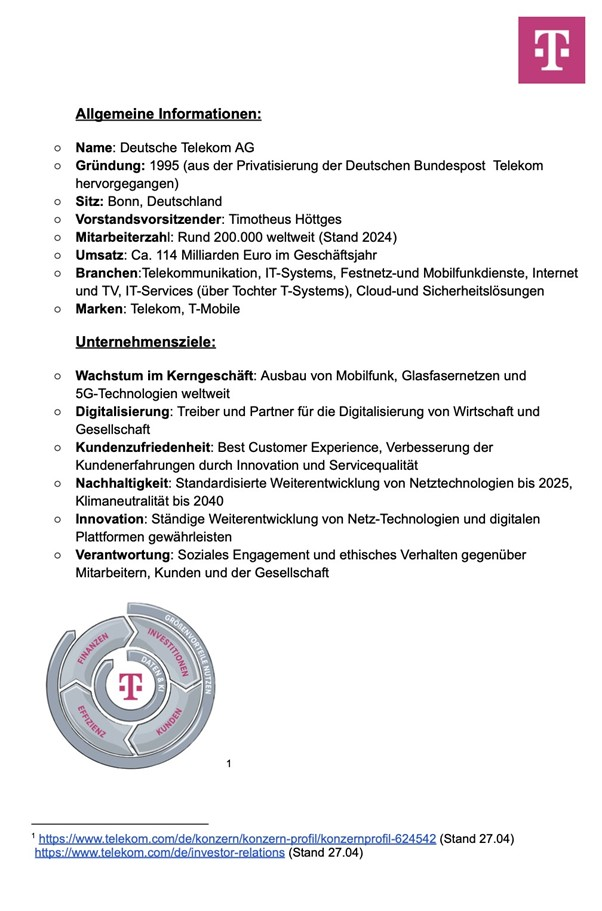
\includegraphics{images/Bild1.jpg}
	\end{figure}
	\newpage
	%------------------------- Anhang -------------------------
	\newpage
	\section{Anhang}
	[Zusätzliche Materialien wie Interviewleitfäden etc.]
	
	%------------------------- KI-Nutzung -------------------------
	\newpage
	\section{Anhang: Nutzung von Künstlicher Intelligenz}
	\begin{itemize}
		\item \textbf{Tool:} ChatGPT
		\item \textbf{URL:} \url{https://chatgpt.com}
		\item \textbf{Prompt:} „Erstelle eine vollständige LaTeX-Vorlage für eine Gruppenarbeit.“
		\item \textbf{Verwendet durch:} Mika Scheinig, Elija Wendte, Justus Kressmann, Engin Fidansoy, Manar Krenbeh
		\item \textbf{Datum:} 04.07.2025
	\end{itemize}
	\begin{itemize}
		\item \textbf{URL:} \url{https://chatgpt.com/share/682f2a68-37b8-8007-9855-d878bcd54ae3}
		\item \textbf{Prompt:} „Kannst du mir ein konkretes Beispiel für einen überregulierten internen Prozess der Deutschen Telekom nennen?“
		\item \textbf{Verwendet durch:} Mika Scheinig
		\item \textbf{Datum:} 22.05.2025
	\end{itemize}
	
	\begin{itemize}
		\item \textbf{URL:} \url{https://chatgpt.com/c/683721e2-4a9c-8001-b0a1-f2e5a1b3f5f2}
		\item \textbf{Prompt:} „Bitte erläutere die Unterschiede in der Leitungsspanne zwischen standardisierten operativen Bereichen und komplexeren Organisationseinheiten wie der Matrixorganisation bei T-Systems. Wie beeinflusst die Organisationsstruktur die Anzahl der direkt unterstellten Mitarbeitenden, und welche Herausforderungen ergeben sich für Führungskräfte in einer Matrixstruktur?“
		\item \textbf{Verwendet durch:} Justus Kressmann
		\item \textbf{Datum:} 24.05.2025
	\end{itemize}
	
	\newpage
	\section*{Eidesstattliche Erklärung}
	Hiermit versichern wir, dass wir die vorliegende Arbeit selbstständig und nur mit den angegebenen Hilfsmitteln und Quellen angefertigt haben. Alle Stellen, die wörtlich oder sinngemäß aus Quellen übernommen wurden, sind entsprechend kenntlich gemacht. Die Arbeit wurde in gemeinsamer Verantwortung erstellt.
	
	\vspace{2cm}
	Oldenburg, 01. Juni 2025
	
	Unterschriften: \\
	\rule{5cm}{0.4pt} Mika Scheinig \\
	\rule{5cm}{0.4pt} Elija Wendte \\
	\rule{5cm}{0.4pt} Justus Kressmann \\
	\rule{5cm}{0.4pt} Engin Fidansoy \\
	\rule{5cm}{0.4pt} Manar Krenbeh
	
	
	
\end{document}
